% -*-latex-*-

%% This is an example first chapter.  You should put chapter/appendix that you
%% write into a separate file, and add a line \include{yourfilename} to
%% main.tex, where `yourfilename.tex' is the name of the chapter/appendix file.
%% You can process specific files by typing their names in at the
%% \files=
%% prompt when you run the file main.tex through LaTeX.

\chapter{Data Analysis}
\label{Data_Analysis}

In this chapter, we will discuss the data analysis procedures
of Coulomb Sum Rule Experiment (E05110).

%%%%%%%%%%%%%%%%%%%%%%%%%%%%%%%%%%%%%%%%%%%%%%%%%%%%%%%%%%%%%%%%%%%%%%
\section{Optics Calibration}
\label{Optics_Calibration}

The Hall A HRS are two spectrometers each with an identical group of superconducting magnets,
three quadrupoles and a dipole in a QQDQ configuration as mentioned in the previous chapter.
The optics matrix is used to reconstruct the interaction vertex at the target from coordinates
of detected particles at the focal plane. This section will discuss the optics calibration procedure
used to determine the optics matrix elements.

\subsection[Coordinate System]{Coordinate System}
\label{Coordinate_System}
In this section, some coordinate systems used in optics calibration are
introduced. More details of these coordinate systems can be found in .
%~\cite{NIM}.

Note that an reference to an angular coordinate should be taken to refer
to the tangent of the angle.

\subsubsection{Hall Coordinate System(HCS)}

The origin of HCS is at the center of Hall A, which is the intersection of
beamline and vertical symmetric axis of the target system. The z axis is
along the beamline and pointing to the beam dump, the x axis is pointing to
the left of the beam, and the y axis is pointing up (See Figure.~\ref{fig:hcs}).

\begin{figure}
  \begin{center}
	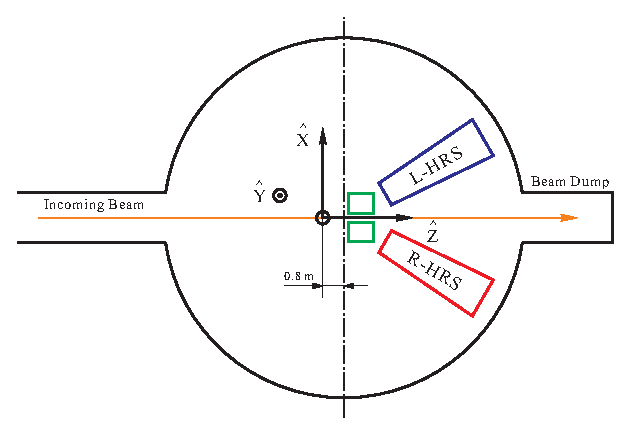
\includegraphics[scale=0.8]{figs/hcs}
  \end{center}
  \caption[Top view of hall coordinate sytem]
  {Top view of hall coordinate system.}
  \label{fig:hcs}
\end{figure}

\subsubsection{Target Coordinate System(TCS)}

Each of the spectrometers has its own TCS coordinate. The z axis of TCS is
along spectrometer center line and perpendicular to the sieve slit surface,
pointing from target. The y axis is going through the origin, pointing to 
the left side of z axis. x axis is pointing down vertically.(See
Figure.~\ref{fig:tcs}) In ideal case,
the origin of TCS is pointing to the Hall center, the origin of TCS and HCS
are same. In the experiment, the HRS central ray is not ideally pointing to
the Hall center, there is a horizontal shift $D_y$ and vertical shift $D_x$.
These shifts are measured in survey. The distance from TCS origin to the
center of collimator is defined as a constant, L. The in-plane angle of a
trajectory $\theta_{tg}$ is defined as $\frac{x_{sieve}}{L}$, and the out-of
-plane angle $\phi_{tg}$ is defined as $\frac{y_{sieve}}{L}$.

\begin{figure}
  \begin{center}
	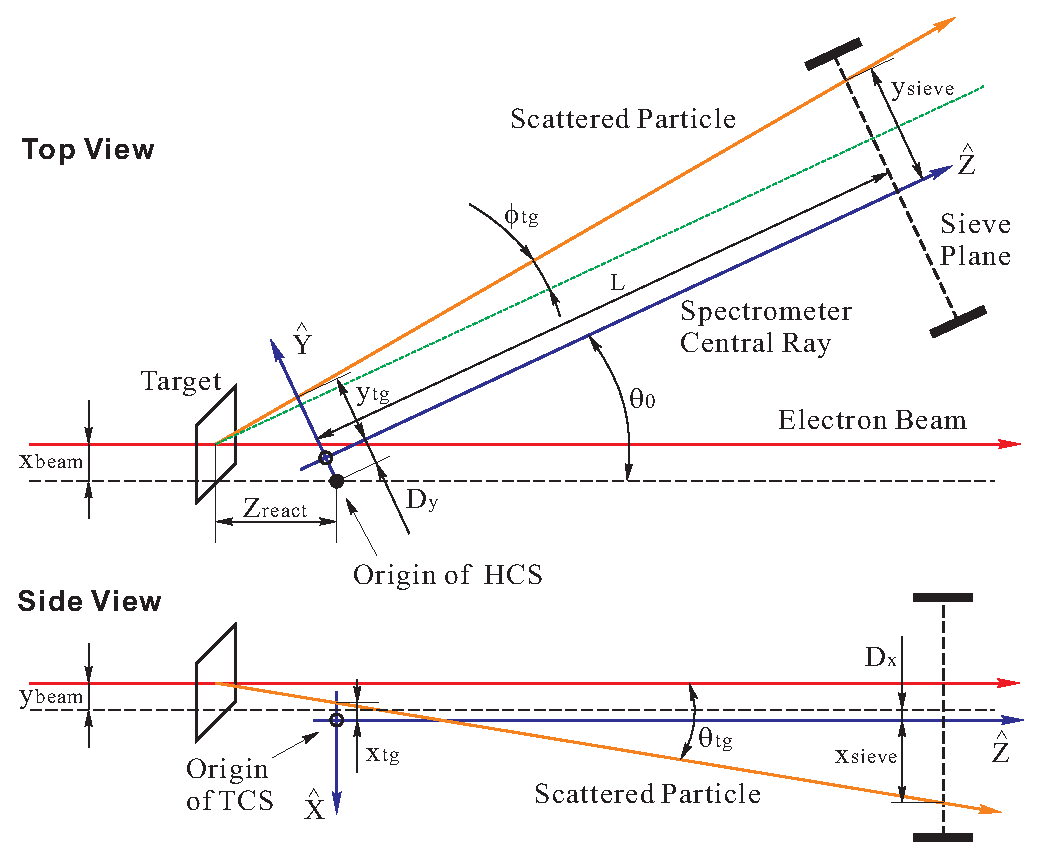
\includegraphics[scale=0.8]{figs/tcs}
  \end{center}
  \caption[Top and side view of target coordinate sytem]%
  {Top and side view of target coordinate sytem.}
  \label{fig:tcs}
\end{figure}

\subsubsection{Detector Coordinate System(DCS)}

The origin of DCS is defined by the wire 184 of VDC U1 plane and wire
184 of VDC V1 plane's projection on U1 plane. The $z$ axis is perpendicular
to the VDC plane, the $x$ axis is along the long symmetry axis and pointing
to the dispersive direction (See Figure.~\ref{fig:dcs}).
The coordinate of the detector vertex can be calculated from the
intersection points on four VDC planes(U1, V1, U2, V2):
  \begin{align}
  \tan (\eta_1) = \frac{p_{U2} - p_{U1}}{d2} \\
  \tan (\eta_2) = \frac{p_{V2} - p_{V1}}{d2} \\
  \theta_{det} = \frac{1}{\sqrt{2}} (\tan(\eta_1)+\tan(\eta_2)) \\
  \phi_{det} = \frac{1}{\sqrt{2}} (-\tan(\eta_1)+\tan(\eta_2))  \\
  x_{det} = \frac{1}{\sqrt{2}}{p_{U1}+p_{V1}-d_1 \tan(\eta_2)}  \\
  y_{det} = \frac{1}{\sqrt{2}}{-p_{U1}+p_{V1}-d_1 \tan(\eta_2)} 
  \end{align}

\begin{figure}
  \begin{center}
	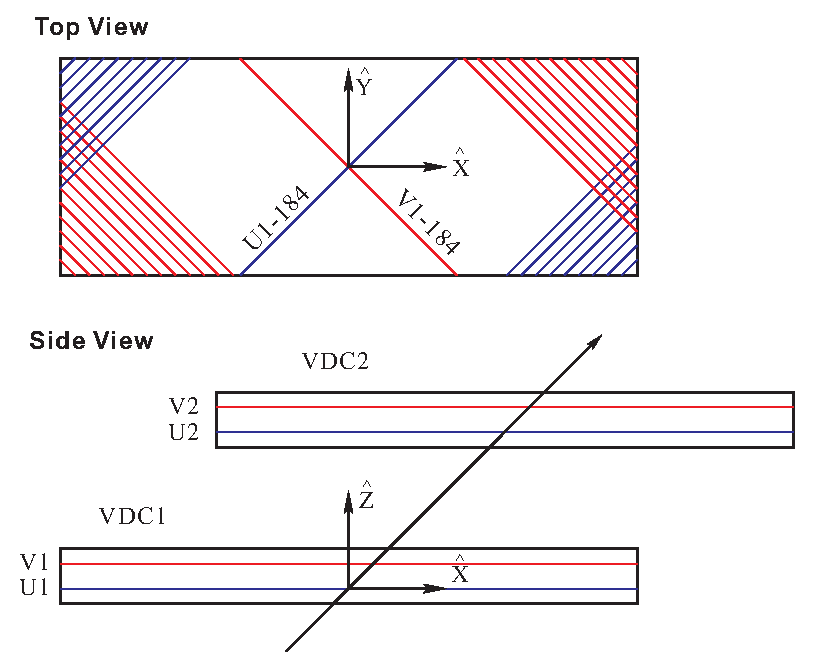
\includegraphics[scale=0.8]{figs/dcs}
  \end{center}
  \caption[Top and side view of detector coordinate sytem]%
  {Top and side view of detector coordinate sytem.}
  \label{fig:dcs}
\end{figure}

\subsubsection{Target Transport Coordinate System(TRCS)}

The TRCS is generated by rotating DCS clockwise along its $y$ axis by
45$^\circ$ (see Figure.\ref{fig:trcs}). So the $z$ axis of TRCS will
coincides with the central trajectory of the spectrometer in the ideal case.
It is a middle step from DCS to Focal Plane Coordinate(FCS) which will be 
described in next section. The transform from DCS variable to TRCS variables
can be expressed by:

\begin{figure}
  \begin{center}
	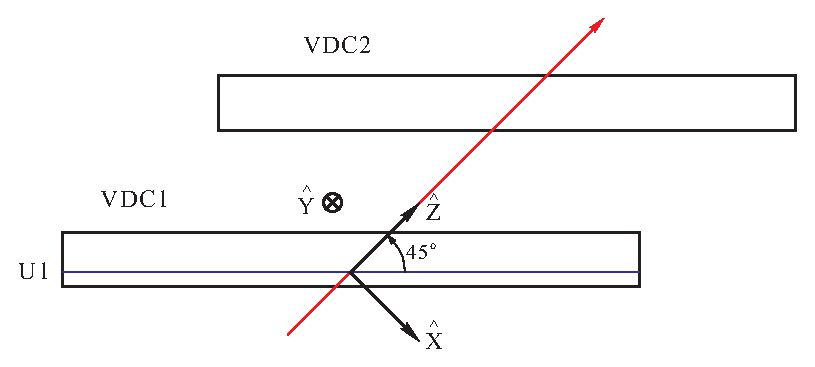
\includegraphics[scale=0.8]{figs/trcs}
  \end{center}
  \caption[Transport coordinate sytem]%
  {Transport coordinate system.}
  \label{fig:trcs}
\end{figure}

\begin{align}
x_{tra}     = x_{det}\cos(\rho_0)(1+\theta_{tra}\tan(\rho_0)) \\  
\theta_{tra}= \frac{\theta_{det}+\tan(\rho_0)}{1-\theta_{det}\tan(\rho_0)} \\  
y_{tra}     = y_{det}+\sin(\rho_0)\phi_{tra}x_{det} \\ 
\phi_{tra}  = \frac{\phi_{det}}{\cos(\rho_0)(1-\theta_{det}\tan(\rho_0))}
\end{align}

where $\rho_0$ = 45$^\circ$ is the rotation angle.

\subsubsection{Focal Plane Coordinate System(FCS)}

Because the focusing of the dipole in HRS magnet system, particles
from different scattering angle will be focused at focal plane. So the
relative momentum $\delta$ (defined in equation ~\ref{equ:dp}) mostly
depends on the location in dispersive direction, $x_{det}$. 

\begin{equation}
\delta = \frac{p-p_0}{p_0}
\label{equ:dp}
\end{equation}

FCS is a rotated coordinate system,
it is generated by rotating the DCS for a varying angle, $\rho(x_{tra})$,
so the new $\hat{z}$ axis is along to the local central ray, which has
$\theta_{tg}$=0 and $\phi_{tg}$=0 (see Figure.~\ref{fig:fcs}).
With this rotation, the $\theta_{fp}$ is small for all points on focal
plane and approximately centered around $\theta_{fp}$=0.
This will ensure the expansion of the optics matrix will converge faster
during the optimization procedure.

The FCS variables can be expressed as: 

\begin{align}
x_{fp} = x_{tra}
\tan(\rho) = \Sigma t_{i000} x_{fp}^i \\
y_{fp} = y_{tra} - \Sigma y_{i000} x_{fp}^i \\
\theta_{fp} = \frac{x_{det}+\tan(\rho)}{1-\theta_{det}\tan(\rho)} \\
\phi_{fp} = \frac{\phi_{det}-\Sigma p_{i000}x_{fp}^i}{\cos(\rho_0)-\theta_{det}\sin(\rho_0)} 
\end{align}

Here $t_{i000}$, $y_{i000}$, $p_{i000}$ are important optics matrix elements
 that will be discussed below.

\begin{figure}
  \begin{center}
	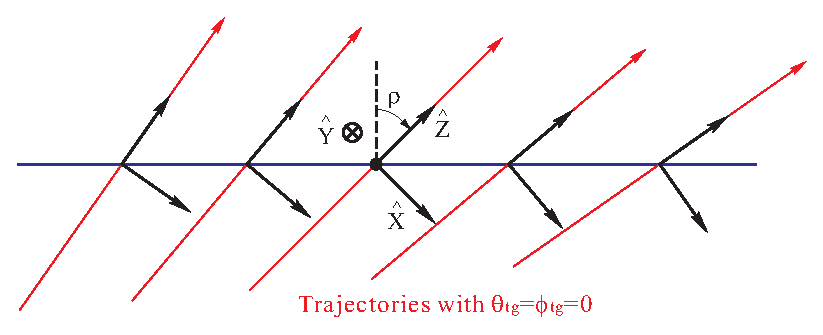
\includegraphics[scale=0.8]{figs/fcs}
  \end{center}
  \caption[Focal coordinate sytem]%
  {Focal coordinate system.}
  \label{fig:fcs}
\end{figure}

% matrix,
% mid-plane symmetry
%
\subsection[Optimization Procedure]{Optimization Procedure}

The DCS variable $x_{det}$, $y_{det}$, $\theta_{det}$, $\phi_{det}$ are
directly measured in experiment, and transformed to focal plane variables
$x_{fp}$, $y_{fp}$, $\theta_{fp}$, $\phi_{fp}$.
%To reconstruct the target variables, we apply a matrix on the focal plane variables.
The optics matrix method provides a point-to-point mapping between focal plane
variables and the target variables, $\theta_{tg}$, $\phi_{tg}$, $y_{tg}$ and $\delta$.

In the optics calibration, the $x_{tg}$ is always set to be zero, and an extended target
correction depend on $beam_{x}$ is applied to $\theta_{tg}$ and $\delta$ in reconstruction.

The first order of optics matrix can be expressed as:

\begin{equation} \label{1st_order_matrix}
  \left(
  \begin{matrix} \delta \\ \theta \\ y \\ \phi \end{matrix}
	\right)_{\mathrm{tg}} = \left(
	\begin{matrix}
	  \left<\delta|x\right> & \left<\delta|\theta\right> & 0 & 0 \\
	  \left<\theta|x\right> & \left<\theta|\theta\right> & 0 & 0 \\
	  0 & 0 & \left<y|y\right> & \left<y|\phi\right> \\
	  0 & 0 & \left<\phi|y\right> & \left<\phi|\phi\right>
	\end{matrix}
  \right)
\left(\begin{matrix} x \\ \theta \\ y \\ \phi \end{matrix}
  \right)_{\mathrm{fp}}.
\end{equation}

The optics matrix used in experiment has a more complicated form: a set of tensors
$D_{jkl}$, $T_{jkl}$, $Y_{jkl}$ and $P_{jkl}$ transform the focal plane variables to
target plane variables as:

\begin{align}
\delta = \sum\limits_{j,k,l} D_{jkl} \theta_{fp}^{j} y_{fp}^{k} \phi_{fp}^{l} \\
\theta_{tg} = \sum\limits_{j,k,l} T_{jkl} \theta_{fp}^{j} y_{fp}^{k} \phi_{fp}^{l} \\
y_{tg} = \sum\limits_{j,k,l} Y_{jkl} \theta_{fp}^{j} y_{fp}^{k} \phi_{fp}^{l} \\
\phi_{tg} = \sum\limits_{j,k,l} P_{jkl} \theta_{fp}^{j} y_{fp}^{k} \phi_{fp}^{l}
\end{align}

where the tensors  $D_{jkl}$, $T_{jkl}$, $Y_{jkl}$ and $P_{jkl}$ are polynomials in $x_{fp}$.
For example:

\begin{align}
\delta = \sum\limits_{j,k,l} D_{jkl} \theta_{fp}^{j} y_{fp}^{k} \phi_{fp}^{l} \\
D_{jkl} = \sum\limits_{i=0} C_{i,j,k}^D x_{fp}^i 
\end{align}

where $C_{i,j,k}^T$ are the optics matrix elements of $\theta_{tg}$.
The optics matrix elements power of  $x_{fp}$, $\theta_{fp}$, $y_{fp}$, $\phi_{fp}$ is 
up to third order. The optics optimization is a method to determine the optics matrix
elements using the optics calibration data. The optimization procedure is described in 
the next section.

\subsection{Experimental and Optimization Procedure}
The optics calibration requires sets of data with wide coverage on the entire acceptance
of spectrometer, which includes $\delta$ for momentum, $\theta_{tg}$ and $\phi_{tg}$ for solid
angle and $y_{tg}$ for reaction position. 
These target variables for calibration data should be precisely determined by methods including:
survey of sieve-slit collimator and spectrometer for $\theta_{tg}$ and $\phi_{tg}$, survey of foil target 
for $y_{tg}$, and some well-known physics process like elastic scattering for $\delta$.

To optimize $\theta_{tg}$, $\phi_{tg}$ and $y_{tg}$, a multi-foil optics target is used,
with a fixed energy, raster-off electron beam. The 7 carbon foils of the optics target
are aligned along the beam line to cover the $y_{tg}$ acceptance, from $z=$-12 cm to $z=$+12 cm,
with a separation of 4 cm. So the $z_{react}$ can be determined by $z$ coordinate of survey result of the 
target foils. The $x_{beam}$ and $y_{beam}$ of interaction point in HCS coordinate can
be determined by BPM. A sieve slit collimator is inserted before the entrance of first quadrupole
of the spectrometer. A figure of the sieve slit is shown in Figure ?.
The holes on the sieve slit are placed in a grid pattern, and the large holes are used to determine
the orientation of the image at the focal plane. 

The in-plane angle $\phi_{tg}$ and out-of-plane angle $\theta_{tg}$ for each sieve-slit hole can be
expressed as:

\begin{align}
\phi_{tg}   =
\frac{y_{sieve}+D_y-x_{beam}\cos\theta_0+z_{react}\sin\theta_0}{L-z_{react}\cos\theta_0-x_{beam}\sin\theta_0}\\
\theta_{tg} = \frac{x_{sieve}+D_x+y_{beam}}{L-z_{react}\cos\theta_0-x_{beam}\sin\theta_0}
\end{align}

where $\theta_0$ is the spectrometer central angle, $D_x$ and $D_y$ are the vertical and horizontal
mis-pointing of the spectrometer central ray from the HCS origin, $L$ is the distance from the
TCS origin to the sieve slit. $\theta_0$, $L$, $D_x$ and $D_y$ can be determined from survey
of spectrometer and sieve slit. The spatial coordinates $x_{tg}$ and $y_{tg}$ can be expressed by:

\begin{align}
x_{tg} = x_{sieve} - L \theta_{tg} \\
y_{tg} = y_{sieve} - L \phi_{tg} 
\end{align}

The momentum calibration use the elastic scattering to determine the momentum of the detected
particle. It requires precise measurement of spectrometer central momentum and beam energy.
The scattering momentum can be expressed as:

\begin{equation}
P(M,\theta) = E' = \frac{E}{1+\frac{E}{M}(1-\cos\theta)}
\end{equation}

where E is the beam energy, M is the target mass and $\theta$ is the scattering angle.
Because the solid angle acceptance covers a wide $\theta_{tg}$ and $\phi_{tg}$ range,
the scattering angles of the electrons passing through different sieve holes are different.
The elastic peak will be broadened and this effect becomes larger for lighter target nucleus.
So a new variable $\delta_{kin}$ is defined to remove the angular dependence of $\delta$ :

\begin{equation}
\delta_{kin} = \delta - \frac{P(M,\theta_{scat})-P(M,\theta_0)}{P0}
\end{equation}

where the scattering angle $\theta_{scat}$ and $\theta_0$ is the central angle of the spectrometer. 
To cover the $\delta$ acceptance of the spectrometer, several different central momentum $P_0$ values
are set during the optics calibration, which is called "delta scan".

The scattered electrons will pass through target foils and several windows before entering spectrometer,
so the energy loss of the scattered electrons due to radiative effect is considered as a correction to
$\delta$.

For optimization of optics matrix, the target variables  $\delta$, $\theta_{tg}$, $\phi_{tg}$ and $y_{tg}$
calculated from survey or elastic scattering peak are taken as the true value.

\begin{equation}
\sigma^2(x) = \sum\limits_{s=1}^{N}  (x^{recon} - x^{survey})^2 
\end{equation}

where $N$ is total number of events measured for optics calibration, x can be any target variables
$\delta$, $\theta_{tg}$, $\phi_{tg}$ and $y_{tg}$, $x^{recon}$ is the target variable 
reconstructed by the optics matrix, $x^{survey}$ is the reference target variable calculated from
survey results and elastic scattering peak. 
The optimization begin with an initial optics matrix generated by magnetic field simulation SNAKE.
The core of the optimization package is the TMinuit package of ROOT.
The package also contain scripts to make graphic cuts and select events for optimization.

\subsection[Optics Results]{Optics Results}
In this section, the optimization results are discussed. The data collected with beam energy 1.1 GeV
at $\theta_0$ = 14.6 degree is taken as an example.

The angular components of the optics matrix are optimized first.
The optimized matrix is used to reconstruct the target variables. The sieve pattern is generated by
the projection of the reconstructed $\theta_{tg}$ and $\phi_{tg}$ from the interaction point to the sieve
slit plane. The sieve pattern for the 1.1 GeV data is shown in Figure ?.
The nominal position of the sieve holes are indicated by the cross points of the grids in the plots.
The resolution of $\theta_{tg}$ and $\phi_{tg}$ are $~1\times 10^{-4}$ mrad and $~ 0.5 \times 10^{-4}$ mrad.

Next step is the momentum calibration. The $\delta_{kin}$ calibration results for 1.1 GeV data are
shown in Figure ?. The nominal position of the $\delta_{kin}$ are indicated by magenta lines for each
delta scan configuration. The resolution of each $\delta_{kin}$ peak is $~ 2 \times 10^{-4}$. 

The $y_{tg}$ calibration results are shown in Figure ?. The nominal position of the optics foils are
indicated by red lines for each foil. The resolution of $y_{tg}$ of foils are $~1 mm$.


%%%%%%%%%%%%%%%%%%%%%%%%%%%%%%%%%%%%%%%%%%%%%%%%%%%%%%%%%%%%%%%%%%%%%%%%
\section{Acceptance of HRS spectrometer}

Because the limited aperture of HRS spectrometer, the spectrometer can only detect scattered electrons
in a certain range of $\theta_{tg}$, $\phi_{tg}$, $\delta$ and $y_{tg}$.
The acceptance of spectrometer can be defined as the window of $\theta_{tg}$, $\phi_{tg}$, $\delta$ and $y_{tg}$ (The foil target only has acceptance in first three variables, the $y_{tg}$ acceptance
is used only for extended target) in which scattered electrons can pass through all the magnets of the
spectrometer and  be detected at focal plane.
In ideal case, the spectrometer would accept all the particles if they are inside the aperture of
spectrometer and reject particles outside aperture.
But in reality, the spectrometer's geometrical aperture is more complicated than a hypercube of 
the five target variables, and the multiple scattering and resolution of the VDC wire chambers will smear
out the boundaries.
So a more proper definition of acceptance is a probability function depend on target variables,
acc($\theta_{tg}$, $\phi_{tg}$, $\delta$, $y_{tg}$). The value  is the 
probability of scattered electrons with certain target variables can reach focal plane.

\subsection{SAMC simulation}
A Monte Carlo simulation package called the Single Arm Monte Carlo (SAMC), is used to study 
the acceptance of spectrometer. The SAMC was originally written in Fortran by  A. Deur and converted
into ROOT/C++ by Huan Yao. A detailed description of the SAMC is given below:

\begin{itemize}
\item Trial events are generated at the target with uniform distribution in $(\delta,\theta_{tg},\phi_{tg},y_{tg})$.
\item
Since each electron pass through target and a few windows, the radiative effects due to the bremsstrahlung
and ionization, and multiple scattering are taken into consideration (The windows and other materials are
listed below in table ?).

\item The SAMC uses a set of forward propagation matrix which is generated by SNAKE simulation
and MUDIFI fit package. The position of each event is checked at every aperture in the spectrometer.

\item The events pass through all the aperture cuts in spectrometer are transported to VDC wire plane.
They are randomly smeared according to the VDC resolution $\sigma_x$ = $\sigma_y$ = 100 $\mu m$,
$\sigma_\theta$ = $\sigma_\phi$ = 0.3 mrad. 

\item All the events reach the focal plane are reconstructed back to the target with reverse matrix.

\end{itemize}

\subsection{Acceptance}

The acceptance used in this analysis are four dimensional acceptance. The projection of the acceptance
on $dp$ and $y_{tg}$ is shown in Figure ?. 

\subsection{Overlap smoothing of acceptance}
Because the forward matrix cannot perfectly describe the magnet field at the edge, the acceptance
at the edge of $dp$ needs to be corrected properly. In experiment, a serial of runs with 
?????????????????????????????

%%
%%%%%%%%%%%%%%%%%%%%%%%%%%%%%%%%%%%%%%%%%%%%%%%%%%%%%%%%%%%%%%%%%%%%%%%%
%\section{BCM calibration}
%Beam Current Monitor (BCM) is done in two steps: 
%
%\subsection{EPICS calibration}
%EPICS calibration provides the absolute beam current measurement.
%This calibration use OLO2 caivity monitor and Faraday cup at the accelerator
%injector section during the calibration run.
%
%During the calibration run, the electron beam only goes to Hall A. The $I_{Faraday}$,
%$I_{OLO2}$ and the average voltage level of BCM cavities (upstream $V^u$ and downstream $V^d$)
%are measured simultaneously. 
%
%\begin{table}[tb!]
%\begin{tabular}{ccr}
%\hline
%$I_{OLO2}$($\mu$A)            & $I_{Faraday}$($\mu$A)         & $\frac{I_{OLO2}}{I_{Faraday}}$-1(\%) \\ \hline
%59.491 $pm$ 0.245             & 59.318 $\pm$ 0.177            & 0.29                                 \\
%39.160 $pm$ 0.049             & 39.048 $pm$ 0.068             & 0.29                                 \\
%19.594 $pm$ 0.033             & 19.472 $pm$ 0.012             & 0.62                                 \\
%10.810 $pm$ 0.039             & 10.723 $pm$ 0.051             & 0.81                                 \\
%5.038 $pm$ 0.007              & 5.034 $pm$ 0.01               & 0.06                                 \\
%2.171 $pm$ 0.008              & 2.164 $pm$ 0.005              & 0.33                                 \\
%1.017 $pm$ 0.002              & 1.019 $pm$ 0.017              & 0.27                                 \\
%0.542 $pm$ 0.002              & 0.549 $pm$ $6\times 10^{-4}$  & 1.20                                 \\
%0.259 $\pm$ $4\times 10^{-4}$ & 0.263 $\pm$ $5\times 10^{-5}$ & 1.50                                 \\ \hline
%\end{tabular}
%\end{table}
%
%\begin{table}[tb!]
%\begin{tabular}{ccr}
%\hline
%BCM Scaler & Scaler Constant   & Offset \\ \hline
%U1         & 2372.4 $\pm$ 2.4  & 362.5  \\
%U3         & 7294.5 $\pm$ 7.5  & 350.2  \\
%U10        & 22067  $\pm$ 225  & 442.6  \\
%D1         & 2427.9 $\pm$ 2.2  & 160.1  \\
%D3         & 7517.4 $\pm$ 8.7  & 126.7  \\
%D10        & 23485  $\pm$ 286  & 321.1  \\ \hline
%\end{tabular}
%\end{table}
%
%The beam charge can be expressed as:
%\begin{equation}
%Q(\mu \C) = \frac{\mathrm{Scaler}_{U3} - \mathrm{Offset_{U3} \times T}{C_{U3}}
%\end{equation}

%%%%%%%%%%%%%%%%%%%%%%%%%%%%%%%%%%%%%%%%%%%%%%%%%%%%%%%%%%%%%%%%%%%%%%%%
\section{Livetime}
There are two types of deadtime: computer deadtime and electronic deadtime.

\subsection{Electronic Deadtime}
When particles generate signals at the detectors, these signals are sent to the TDC and ADC electronics.
The TDC and ADC cannot process singals continuously: when an event is immediately followed by another
before the detector gate is ready for the latter. The gate opening time is $~$ 100 ns for both LHRS and RHRS.



\subsection{Computer Deadtime}
The computer deadtime is

%%%%%%%%%%%%%%%%%%%%%%%%%%%%%%%%%%%%%%%%%%%%%%%%%%%%%%%%%%%%%%%%%%%%%%%%
\section{PID Efficiency}


%%%%%%%%%%%%%%%%%%%%%%%%%%%%%%%%%%%%%%%%%%%%%%%%%%%%%%%%%%%%%%%%%%%%%%%%
\section{Tracking Efficiency}

Vertical Drift Chambers (VDC) detect hits of scattered electrons and reconstruct tracks through track
reconstruction algorithm.
Under normal conditions, each event leaves only one track in the VDC, but in certain case an event
can have zero track or multi-track.
The inefficiency of VDC wire or failure of track reconstruction may result in zero track events.
In most of the case, the wire inefficiency is less than 0.1\%.
The wire inefficiency cannot be separated from the tracking efficiency and is convoluted into 
the multi-track efficiency.
A multi-track event means an event  with 2 or more tracks reconstructed by VDC.
It can happen when several electron generated secondary particles passing through VDC simultaneously,
or there is noise in VDC.

For most of runs in CSR experiment, the event rate is below 10 kHz and only a small fraction of events ha
s multi-track. For kinematics settings with higher trigger rate, the fraction of multi-track events is also
higher: there are some runs with trigger rate higher than 10 kHz, and the multi-track events
takes more than a few percent in total event number. So a strict treatment is necessary for these runs,
the multi-track events must be examined carefully to determine whether or nor there is a good track among all
the reconstructed tracks.
%We can use the PID and acceptance cut to select a clean sample, and use the energy deposit
%around the each track's trajectory in lead glass to check if an event contains a good track.

The tracking efficiency can be defined as the ratio between good events number with a successful track reconstruction
and total events number.

\begin{equation}
\varepsilon_{VDC} = \frac{N_{good}}{N_{total}}
\end{equation}

where $N_{good}$ is the number of events with events with a successful track reconstruction and checked
by the energy deposit on lead glass calorimeter, $N_{total}$ is the number of events that pass the acceptance
cut and PID cut.

Because the check of multi-track event is very time consuming, in analysis of production runs, we usually only
use events with a single track, so a correction for the loss of multi-track events is necessary:
We redefine the tracking efficiency as the ratio between number of good single track events and number of all
good events: 

\begin{equation}
\varepsilon_{VDC} = \frac{N_{goodsingletrack}}{N_{goodsingletrack}+N_{goodmultitrack}}
\end{equation}

where the $N_{singlegoodtrack}$ is the number of events with good single-track events in the sample,
$N_{multigoodtrack}$ is the number of multi-track events with at least one good track in the sample.

A multi-track event is considered as good event if :
(a) at least one track inside the normal acceptance cut used for this analysis:
$|dp|\leq$ 3.5\%, $|\theta_{tg}| \leq$ 40 mrad, $|\phi_{tg}| \leq$ 20 mrad;
(b) energy deposited in the calorimeter of this track satisfies the PID cuts.
Figure xx shows the acceptance cut used in this analysis.

To get the energy deposition of a track in calorimeter, we need to project the
track trajectory forward onto calorimeter (Because some of the blocks of the NaI calorimeter in LHRS was
not responsive during the experiment, this tracking efficiency is only studied on
RHRS, and then applied to LHRS).
Figure xx shows the distribution of energy deposition in 2 layers of calorimeter (shower and preshower)
for two-tracks events. The  
%%%%%%%%%%%%%%%%%%%%%%%%%%%%%%%%%%%%%%%%%%%%%%%%%%%%%%%%%%%%%%%%%%%%%%%%
\section{Center-of-bin Correction}

With an angular cut of $|\theta_{tg}|\leq$ 40 mrad,  $|\phi_{tg}| \leq$ 20 mrad, as mentioned previously,
the cross section measured at a certain central spectrometer angle actually is the average of cross section
in the range of acceptance. Because the cross section varied non-linearly within the finite bin of the acceptance,
a center-of-bin correction is applied to correct this finite acceptance effect.

If we know the cross sections very well, for example, the carbon/proton elastic cross section,
we can use the parametrized cross section from phase shift calculation to get a center-of-bin factor, $C_a$:

\begin{equation}
C_a = \frac{\sigma_c}{ \frac{\int \sigma(\theta,\phi,\delta) \times
Acc(\theta,\phi,\delta)}{\int_{\theta,\phi,\delta}Acc(\theta,\phi,\delta) }}
\end{equation}

where $\sigma_c$ and $\sigma(\theta,\phi)$ are the calculated cross sections at the center and at a certain bin ($\theta,
\phi, \delta$) of the acceptance.

For the case of quasi-elastic scattering region, we don't known the exact cross section, the correction is performed
with a calculated cross section from F1F209 model.

%%%%%%%%%%%%%%%%%%%%%%%%%%%%%%%%%%%%%%%%%%%%%%%%%%%%%%%%%%%%%%%%%%%%%%%%
\section{Radiation Correction}
%%\label{C5S4}
The cross section in equation ? is derived to lowest order in fine-structure
constant $\alpha$ including only the amplitude due to exchange of single virtual photon between 
the incident electron and nucleon, which is known as Born approximation. The cross section measured
in electron scattering in experiments have large contribution from higher order process and the 
straggling effect. So the raw cross section need to be corrected to extract Born cross section.
This correction is called "radiative correction". 
In this section, a summary of theory and application of radiative correction is given.

Feynman diagrams of the second order and third order processes are shown in Figure ?.

Will talk about follow topics in this section:
(1) calculate the elastic tradiative tail; (2) quasi-elastic radiative corrections;
(3) radiative correction to elastic data;

\subsection{Elastic Radiative Tail}
Following the formalism of Mo and Tsai and Stein, the cross section for the elastic radiative tail is:

\begin{equation}
\sigma_{el tail} = (\sigma_{int} + \sigma_{ext} + \sigma_{coll}) \cdot F_{soft}
\end{equation}

where $\sigma_{int}$, $\sigma_{ext}$, $\sigma_{coll}$ and $F_{soft}$ represent the internal bremsstrahlung, external bremsstrahlung
, collisional loss and soft photon correction.

\subsubsection{Internal Bremsstrahlung}
When the bremsstrahlung photon emission is during the collision, this process is called internal bremsstrahlung. The
internal bremsstrahlung cross section for elastic scattering can be calculated exactly (to lowest order order of
$\alpha$) is we assume one-photon exchange.


\begin{equation}
\sigma_{int} = \int B_{\mu\nu} T_{\mu\nu} d\Omega_k,
\end{equation}

where $B_{\mu\nu}$ is the internal bremsstrahlung tensor and $T_{\mu\nu}$ is the lepton tensor.



\subsection{Radiative Corrections for Quasi-elastic Data}

\begin{equation}
t_r = \left(\frac{\alpha}{b\pi} \right) \left[ \ln\left(\frac{Q^2}{m_e^2}\right)-1 \right]
\end{equation}

\begin{equation}
\begin{split}
\left( \frac{d^2\sigma}{d\Sigma d\omega} \right)_{exp}  =  \left(\frac{R\Delta E}{E_i}\right)^{bt'_b}
\left(\frac{\Delta E}{E_f}\right)^{bt'_a} \left[1 - \frac{\xi/\Delta E}{1-b(b(t'_a + t'_b))} \right] \tilde{\sigma}(E_i,
E_f) \\
 + \int_{E_{i min}}^{E_i - R\delta E} \tilde{\sigma}(E'_i, E_f) \left( \frac{E_i - E'_i}{RE_f} \right)^{bt'_a} \left(
\frac{E_i - E'_i}{E_i}\right)^{bt'_b} \\
 \times \left[ \frac{bt'_b}{E_i - E'_i} \phi \left( \frac{E_i-E'_i}{E_i} \right) + \frac{\xi}{2(E_i - E'_i)^2} \right]
dE'_i  \\
 + \int_{E_f + \delta E}^{E_{f max}} \tilde{\sigma} (E_i, E'_f) \left( \frac{E'_f - E_f}{E'_f} \right)^{bt'_a} \left(
\frac{R(E'_f - E_f)}{E_i} \right)^{bt'_b} \\
 \times \left[ \frac{bt'_a}{E'_f-E_f} \phi\left(\frac{E'_f - E_f}{E'_f}\right)+\frac{\xi}{2(E'_f - E_f)^2} \right] dE'_f ,
%
\end{split}
\end{equation}

\subsection{Radiative Corrections for Elastic Data}
The radiative correction to the elastic peak has been well studied.
The relation between cross section measured in experiment and the Born cross section is:

\begin{equation}
\left(\frac{d\sigma}{d\Omega}\right)_{exp} = (1+\delta) \left( \frac{d\sigma}{d\Omega} \right)_{Born}
\end{equation}

where $\delta$ is the radiative correction. Higher order corrections are taken into account by replacing
$1+\delta$ with $e^{\delta}$.

The expression of $\delta$ is sum of the external and internal terms.

The internal term include contribution from internal bremsstrahlung, vacuum polarization and nucleus recoil and photon emission: 

\begin{multline}
%\begin{equation}
%\begin{split}
\delta_{int}  =
%\frac{-\alpha}{\pi} \left(
\frac{28}{9} - \frac{13}{6} \ln \left( \frac{Q^2}{m^2_e} \right)  +
\left( \ln \left( \frac{Q^2}{m^2_e} \right) - 1 + 2Z \ln \left( \frac{E_i}{E_f} \right) \right) \\
\times \left[ 2\ln \left( \frac{E_i}{\Delta E} \right) - 3\ln \left( \frac{E_i}{E_f} \right) \right]  \\
-\Phi \left( \frac{E_f-E_i}{E_f} \right)
- Z^2 \ln \left( \frac{E_t}{M_t} \right)
+ Z^2 \ln \left( \frac{M_t E_f}{E_i \Delta E} \right)
\left( \frac{1}{\beta_t} \ln \left( \frac{1+\beta_t}{1-\beta_t} \right) -2 \right) \\
+ \frac{Z^2}{\beta_t} \left\{ \frac{1}{2} \ln\left( \frac{1+\beta_t}{1-\beta_t} \right) \ln\left( \frac{E_t+M_t}{2M_t} \right) 
-\Phi \left[ -\left( \frac{E_t-M_t}{E_t+M_t}\right) \left(  \frac{1+\beta_t}{1+\beta_t} \right)^{\frac{1}{2}} \right]
\right\} \\
- Z \left[ \Phi\left(-\frac{E_t-E_f}{E_f}\right) -\Phi\left( \frac{M_t(E_t-E_f)}{2E_iE_t-M_tE_f} \right)
+ \Phi \left( \frac{2E_i(E_t - E_f)}{2E_i E_t - M_t E_f} \right)  
%+\ln | \frac{2E_i E_t - M_t E_f}{E_f(M_t - 2E_i)} | \ln left( \frac{M_t}{2E_i} \right)
\right]
%\right)
%\end{split}
%\end{equation}
\end{multline}


%%%%%%%%%%%%%%%%%%%%%%%%%%%%%%%%%%%%%%%%%%%%%%%%%%%%%%%%%%%%%%%%%%%%%%%%
\section{Experimental Cross Section}
The goal of E05-110 experiment is to measure the longitudinal and transverse response functions, and 
extract Coulomb Sum to test Coulomb Sum Rule(CSR). To obtain Coulomb Sum with required precision,
it is important to extract the cross section while minimizing the uncertainties. The raw experimental cross
section can be written as:

\begin{equation}
\frac{d\sigma}{d\Sigma d\omega} = \frac{N_{cut}}{(Q/e) \cdot t_{LT} \cdot Acc \cdot \varepsilon \cdot N_{tg}}
\frac{1}{\Delta E' \Delta \Omega}
\end{equation}

\begin{itemize}
\item $N_{cut}$ is the number of events within all electron cut in one bin.

\item $Q/e$ is the number of incident electrons. $Q$ is the total charge which is read from BCM scaler.
$e$ is the charge of a single electron.

\item $t_{LT} = T_{1(3)}/T_{1(3)raw}$ is the Livetime of the detector.
$T_{1(3)}$ are the main trigger event type for right(left) arm.

\item $Acc$ is the spectrometer's acceptance determined from Monte Carlo simulation (SAMC).

\item $\varepsilon$ is the total efficiency $\prod_i \varepsilon_i$ for all detectors:
VDC, scintillator, gas Cerenkov, shower and preshower;

\item $N_{tg}$ is the number of the target particles.  $L\rho$ is the target thickness (in unit of g/cm$^3$),
$N_a = 6.02 \times 10^{23}$ is the Avagadro's number. A is the atomic number of the target.

\begin{equation}
N_{tg} = \frac{L\rho N_a}{A}
\end{equation}

\item $\Delta E = P_0 dp$ is the energy width (in unit of MeV) for the given momentum bin.

\item $\Delta \Omega = \Delta \theta \Delta \phi$ is the solid angle defined by the width of acceptance cuts in
$\theta_{tg}$ and $\phi_{tg}$. In this analysis, cut in $\theta_{tg}$ and $\phi_{tg}$ are $\Delta \theta$ = 80 mrad,
and $\Delta \phi$ = 40 mrad.

\end{itemize}

%%%%%%%%%%%%%%%%%%%%%%%%%%%%%%%%%%%%%%%%%%%%%%%%%%%%%%%%%%%%%%%%%%%%%%%%
\section{Density effect}

The $^{4}$He is in high pressure gas state, and the $^{208}$Pb is
kept in liquid hydrogen. For fluid targets, the local heating generated
by beam current may result in decrease of density near the beam trajectory. 
This localized effect cannot be detected by sensor devices.
This density fluctuation effect can be measured by investigating the 
linearity between the event yield and the beam current using elastic
scattering data.

The density fluctuation depends on two parameters, beam current and beam
size. A higher beam current/smaller beam size will decrease the target
density.  Due to the configuration of the cryogenic target, that the 
cooling enter the target from the top and exit from the bottom, the 
vertical beam size has less effect on target density.

And it is interesting to see the difference between the two kinds of
cryogenic target: the density of $^{4}$He target decrease linearly as
beam current grows, while the liquid hydrogen target has a changing 
slope. The density fluctuation is less than 5\% for this analysis.


%%%%%%%%%%%%%%%%%%%%%%%%%%%%%%%%%%%%%%%%%%%%%%%%%%%%%%%%%%%%%%%%%%%%%%%%
%%\section{Rosenbluth Separation}
%%\label{C5S5}



%\cite{*}

%%%%%%%%%%%%%%%%%%%%%%%%%%%%%%%%%%%%%%%%%%%%%%%%%%%%%%%%%%%%%%%%%%%%%%
% -*-latex-*-
